\documentclass{report}

\usepackage{graphicx}
\usepackage{amsmath}
\usepackage{hyperref}

\begin{document}

\title{Bayesian Modeling of tri-functional crosslinkers to 
elucidate protein complex structures: 26s human proteasome}
\author{Echeverria group}
\date{\today}
\maketitle

\tableofcontents

\chapter{Introduction}
\label{chap:introduction}
Protein complexes play a crucial role in various biological processes. 
Understanding their structures is essential for insights into their functions. 
Bayesian modeling offers a probabilistic framework for inferring protein structures 
from experimental data.
\begin{figure}
\centering
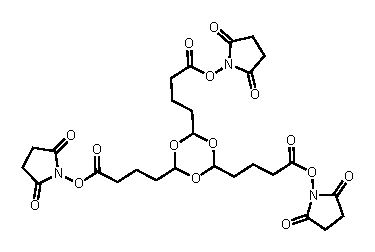
\includegraphics[scale=1.0]{./figures/tri-linker.eps}
\caption{Chemical structure of the tri-functional crosslinker}
\end{figure}

\chapter{Methodology}
\label{chap:methodology}
This section describes the Bayesian modeling approach used in this study. 
It includes details on the data, the probabilistic model, and the 
computational methods employed.

\section{Computational Methods}
Detail the algorithms and software tools used for Bayesian inference, such as Markov Chain Monte Carlo (MCMC) methods.
\begin{figure}[ht!]
    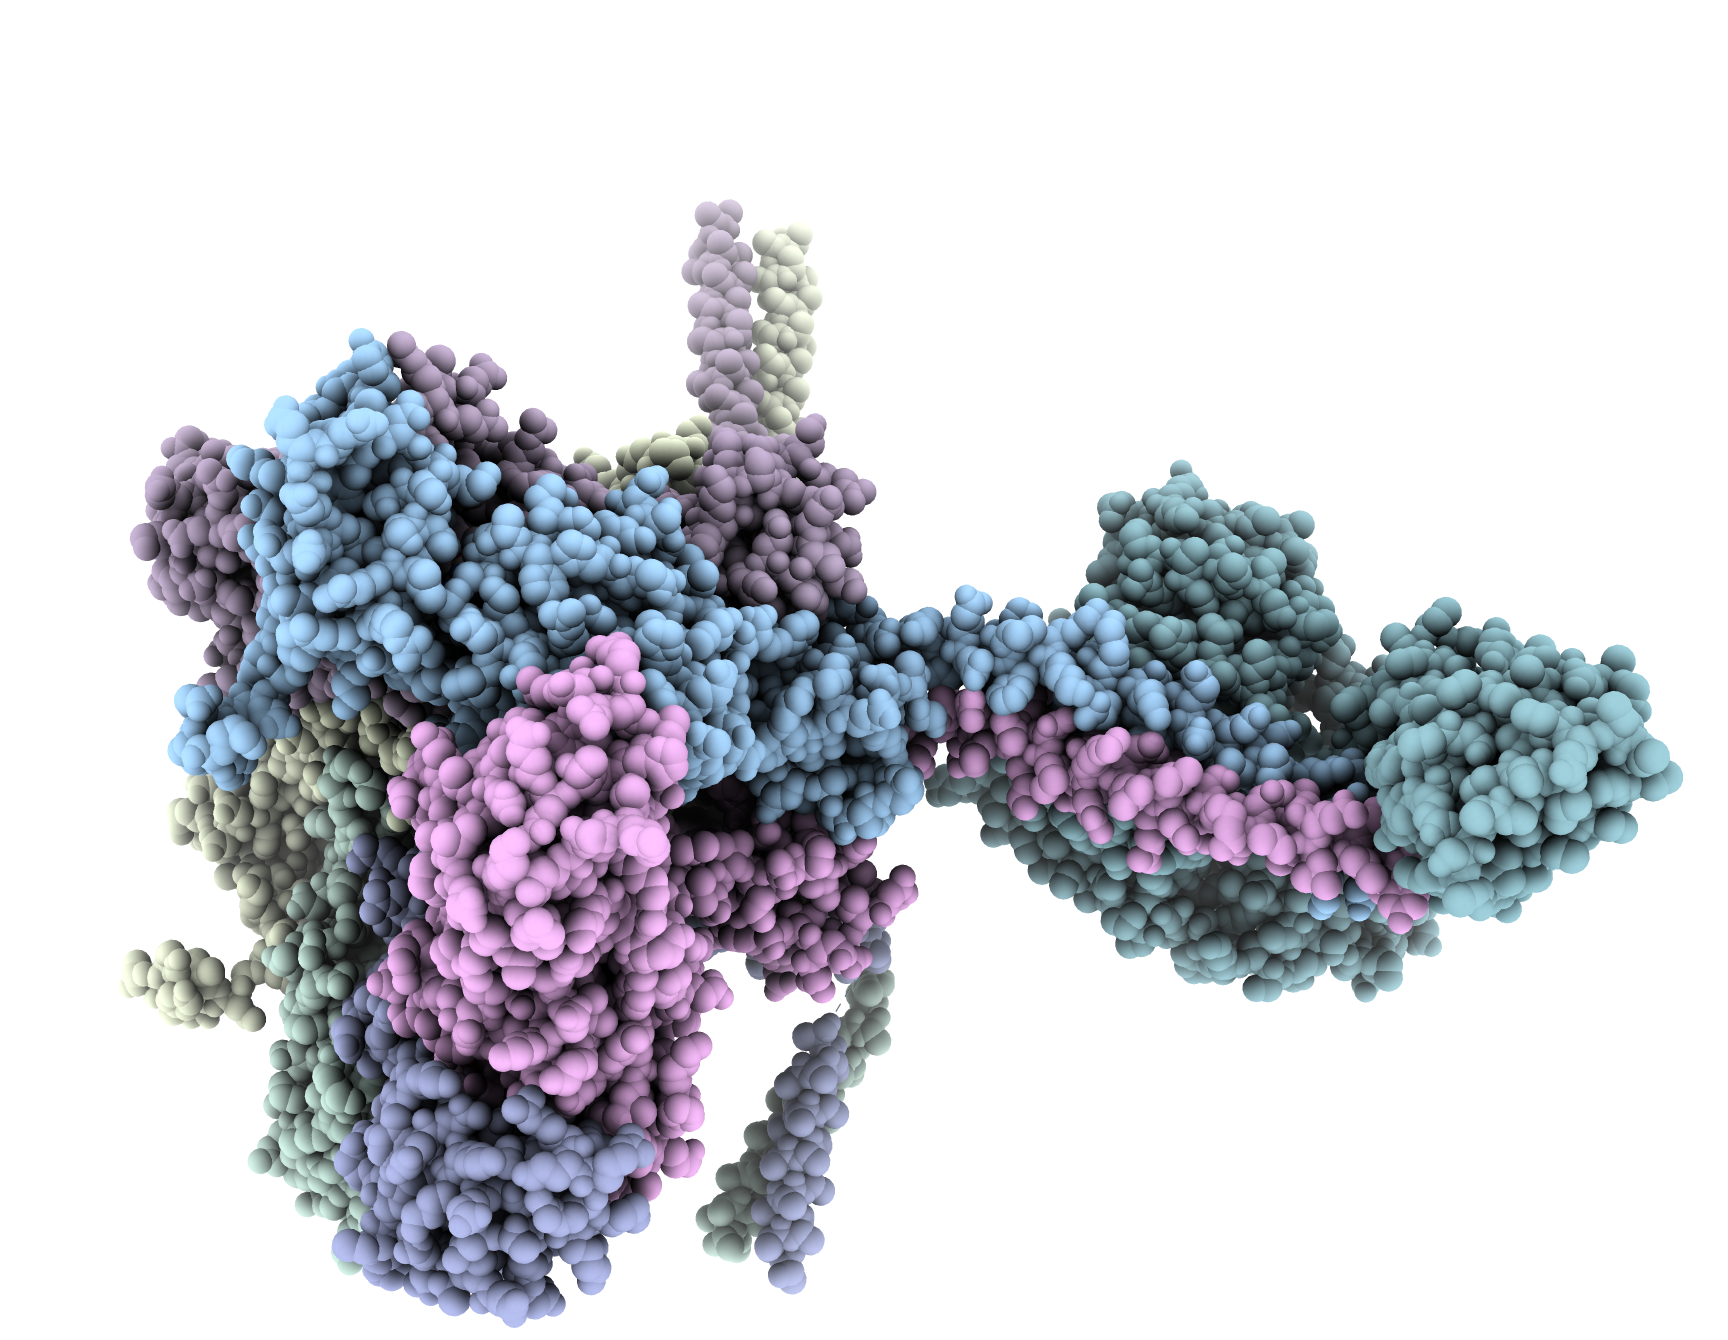
\includegraphics[width=\textwidth]{./figures/base_proteasome_5gjr.png}
    \caption{Subcomplex of the human proteasome, which forms the base. It consists of 
    Rpt1, Rpt2, Rpt3, Rpt4, Rpt5, Rpt6 and Rpn2 subunits.}
\end{figure}
\chapter{Results}
\label{chap:results}
Present the results of the Bayesian modeling. Include figures and tables to illustrate the inferred protein complex structures and any relevant statistical analyses.

\begin{thebibliography}{9}
    \bibitem{example1}
    Author, \textit{Title of the paper}, Journal, Year.

    \bibitem{example2}
    Author, \textit{Title of the book}, Publisher, Year.
\end{thebibliography}

\end{document}

